\section {NetInf Video Streaming Protocol}

\subsection{Introduction}

The purpose of this draft is to outline a design and protocol specification for enabling of streaming and chunking data within the current and existing netinf architecture.

\subsubsection{Proposed method of retrieving chunked NDOs}

The stream source will PUBLISH an NDO containing the filename as content. The object is marked as streaming video in the meta data. It also contains a locator to the stream source.

In order to access the stream, a receiver will first perform a NetInf-GET on the above filename object in order to retrieve the locator. 

In the next step the client can get the chunks. By replacing the hash algorithm in the NDO-name with \_demo\_ and sending a NetInf-GET to the source, the stream provider will return the octets of the most recent chunk and the chunk number in the metadata. This implies that the regular hash validation has been disabled.

For further chunks, the receiver will increment the chunk number and append it to the locator.\\

\textbf{Publish}\\
\begin{verbatim}
 ni:///sha-256;WkOCMB2aEQHrARjTldfhRE5OgZkZmCHzokcoVMnfp2Y

Get latest chunk
 ni:///demo;WkOCMB2aEQHrARjTldfhRE5OgZkZmCHzokcoVMnfp2Y

Get first chunk, append a 0 to the end of the hash
 ni:///demo;WkOCMB2aEQHrARjTldfhRE5OgZkZmCHzokcoVMnfp2Y0

Get the 32th chunk, append 32 to the end of the hash
 ni:///demo;WkOCMB2aEQHrARjTldfhRE5OgZkZmCHzokcoVMnfp2Y32
\end{verbatim}
 
If the receiver also acts as a cache, it will send a PUBLISH with the filename object and a locator pointing to itself to the NRS.
\\

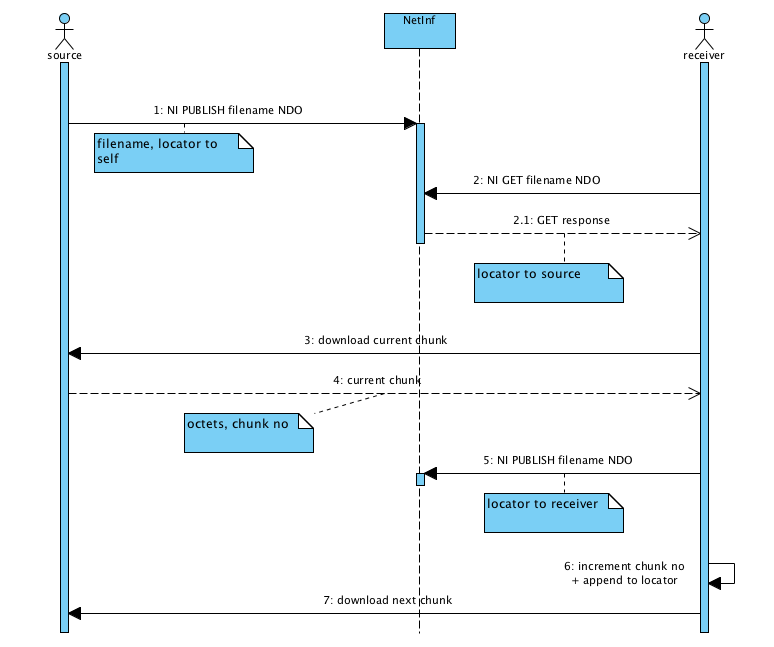
\includegraphics[scale=0.5]{./img/sequence_diagram_streaming.png}

\subsubsection{Testing criteria} 

For a simple test setup, in addition to our NetInf node, we need a receiving and a publishing client. A more sophisticated test could involve multiple receivers, to demonstrate the caching.

A use case we can use for testing is one where our source of the content is a pre-encoded video file of a particular size.

In the example below we will assume a video file of 700 megabytes.

A client (Publisher) will have a default chunk size which we will use to chunk up the source file. For example we will use 1 megabyte chunk size.

We can calculate from the Publisher that we will have 700 chunks, of 1 megabyte each numbered 0-699. 

A second client (receiver) knowing the name of the video file will then perform a GET request within the NetInf node (to keep things simple, we assume it knows the object's name already).

The client will now start generating consecutive GET's with the sequence numbers constantly increasing and expect to receive the appropriate chunk.

Also poll the NRS for new locators, to reduce the load of the network.

Until the GET's generate a 404 because the unique sequence number has increased past a chunk number that is not published.

\subsubsection{Extra notes}

Chunk size is going to be a configurable option in the publishing client.

The polling logic needs to be implemented in the client, that is how often the receiver should get a new chunk or check if a new chunk exists.  